\newpage
\section{22. 括号生成}
\label{leetcode:22}

\subsection{题目}

给出 n 代表生成括号的对数,请你写出一个函数,使其能够生成所有可能的并且有效的括号组合。

例如,给出 n = 3,生成结果为:

\begin{verbatim}
  [
    "((()))",
    "(()())",
    "(())()",
    "()(())",
    "()()()"
  ]
\end{verbatim}

\subsection{参考题解,暴力递归}

n = 3,那么字符串的长度 = 2 * n = 6,每一个字符都可以是 
\verb|'('| 或者 \verb|')'|,我们遍历出所有的情况,然后
最后加上合法性判断。

我们另字符串的长度为 n,那么因为每个字符都有两种可能性,
所以时间复杂度为 $\underbrace{2*2*\cdots*2}_{n}$,即 O(2$^{n}$)。

你可能还是不太理解,你可以看下面这个状态树,
你会发现,我们要找的答案都是在最下面的叶子节点。
那这个题目就可以转化为树的遍历,然后遍历到叶子节点,
判断下是否合法,把合法的叶子节点保存下来就是最终的答案了。

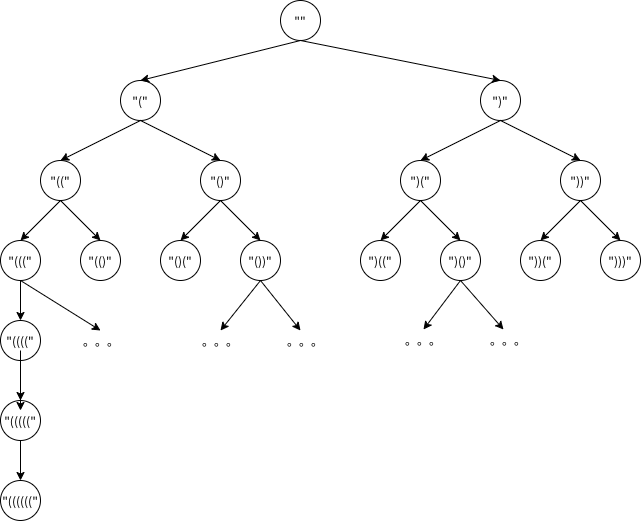
\includegraphics[width=150mm,height=100mm]{images/leetcode/leetcode_22.png}

下面给出深度优先遍历的代码。

\begin{verbatim}
/**
 * @param {number} n
 * @return {string[]}
 */
var generateParenthesis = function(n) {
  let result = [];
  recursion(2*n, 0, result, "");
  return result;
};

function recursion(n, i, result, strs) {
  if (i === n) {
    if (isValid(strs)) {
      result.push(strs);
    }
    return;
  }

  recursion(n, i + 1, result, strs + "(");
  recursion(n, i + 1, result, strs + ")");
}

var isValid = function(s) {
  let stack = [];
  for (let c of s) {
    if (c === '(') {
      stack.push(')');
    } else if (c !== stack.pop()) {
      return false;
    }
  }
  return stack.length === 0;
};
\end{verbatim}

\subsection{参考题解,剪枝}

剪枝的意思就是在递归的过程中就把一些很明显不合法的分支去掉,
以达到减少遍历的时间。如果剪枝能够把所有的不合法分支都去掉,
那剩下的就是合法的。如果剪枝只能去掉部分不合法分支,那最后
还是需要加上字符串的合法性判断。

认真观察上面的那个状态树的话,你会发现有的分支很明显是不合法的,
比如根节点的右儿子,很明显这个分支的所有情况都是不合法的,我们
如果能够把这个去掉,就可以加快遍历的速度。但是时间复杂度依然是 O(2$^{n}$)。

\begin{verbatim}
/**
 * @param {number} n
 * @return {string[]}
 */
var generateParenthesis = function(n) {
  let result = [];
  recursion(result, 0, 0, n, "");
  return result;
};

function recursion(result, left, right, n, strs) {
  if (left === n && right === n) {
    result.push(strs);
    return;
  }
  if (left < n) {
    recursion(result, left + 1, right, n, strs + "(");
  }
  if (right < left) {
    recursion(result, left, right + 1, n, strs + ")");
  }
}
\end{verbatim}
